\documentclass[a4paper,10pt]{article}

% Paquetes requeridos
\usepackage[utf8]{inputenc}
\usepackage[spanish]{babel}
\usepackage{csquotes}
\usepackage{amsmath, amssymb, amsfonts}
\usepackage{graphicx}
\usepackage[style=apa, backend=biber, natbib=true, language=spanish, url=true]{biblatex}
\usepackage{tocloft} % Para personalizar el índice
\usepackage[left=3.5cm,right=2.5cm,top=3.5cm,bottom=3.8cm]{geometry}
\usepackage{setspace} % Espaciado
\usepackage{titlesec} % Para personalizar los títulos
\usepackage{fancyhdr} % Para personalizar encabezados y pies de página
\usepackage{newtxtext}

\pagestyle{fancy}
\fancyhf{} % Limpia encabezados y pies de página
\renewcommand{\headrulewidth}{0pt} % Elimina la línea del encabezado

\addbibresource{referencias.bib}
\DeclareLanguageMapping{spanish}{spanish-apa}
% Configuraciones
\setlength{\parskip}{6pt} % Espacio entre párrafos
\setstretch{1.15} % Espacio entre líneas

\renewcommand{\cftsecleader}{\cftdotfill{\cftdotsep}} % Para puntos en el índice

% Estilos para títulos y subtítulos
\titleformat{\section}
{\normalfont\fontsize{12}{15}\bfseries}{\thesection}{1em}{}
\titleformat{\subsection}
{\normalfont\fontsize{10}{13}\bfseries}{\thesubsection}{1em}{}
\titleformat{\subsubsection}
{\normalfont\fontsize{10.5}{13}\bfseries}{\thesubsubsection}{1em}{}

\usepackage[hypertexnames=false, colorlinks=true, 
linkcolor=blue, 
citecolor=blue, 
urlcolor=blue, 
linkbordercolor={1 1 0}, 
citebordercolor={1 1 0}, 
urlbordercolor={1 1 0}, 
filecolor=blue, 
pdfborderstyle={/S/U/W 1}]{hyperref}

% Inicio del documento
\begin{document}
	\pagestyle{empty}
	% Carátula
	\begin{titlepage}
		\centering
		\vspace*{1.5cm}
		
\includegraphics[width=0.3\textwidth]{unerlogo.png}
		\linebreak
		{\fontsize{14}{17}\bfseries Trabajo integrador: Metaverso y Solidity\par}
		{\small Martín Borgo\par}
		{\small Leandro Molina\par}
		{\normalsize Universidad Nacional de Entre Ríos\par}
		{\normalsize Facultad de Ciencias de la Administración\par}
		{\normalsize Licenciatura en Sistemas \par}
		{\small \href{mailto:martinborgo8@gmail.com}{martinborgo8@gmail.com}\par}
		{\small \href{mailto:LeandroRodrigoMolina@gmail.com}{LeandroRodrigoMolina@gmail.com}\par}
		
		% Resumen y palabras clave
		{\small \textbf{Abstract.} Resumen hasta 200 palabras. \par}
		{\small \textbf{Keywords:} Metaverso, Solidity, Contratos inteligentes (Smart Contracts), Blockchain.\par}
	\end{titlepage}
	
	% Índice
	\tableofcontents
	\thispagestyle{empty}
	%Empezamos a escribir
	\section{Introducción}
	\subsection{¿Qué significa “metaverso”?}
	El metaverso, conocido también como universo metafísico o espacio virtual, se refiere a un entorno virtual 3D en línea, donde todos los eventos que ocurren en él se producen en tiempo real y tienen un impacto permanente. La palabra "metaverso" está compuesta por el prefijo "meta", que viene del griego \( \mu\varepsilon\tau\acute{\alpha} \) y significa "más allá" o "después". En el contexto del metaverso, este prefijo se refiere a la idea de un universo que va más allá de lo físicamente conocido. Por otro lado, el final "-verso" proviene del latín "universus", que significa "todo en uno" o "entero". Por lo tanto, el metaverso se puede interpretar como "un universo alternativo" o "más allá del universo", refiriéndose a un espacio virtual en línea autónomo que existe más allá de nuestro universo físico.
	\subsection{Origen e historia del metaverso}
	El término metaverso se popularizó por la novela de Neal Stephenson “Snow Crash”, en esta novela de género ciencia ficción, más específicamente del subgénero Cyberpunk\footnote{El subgénero Cyberpunk se centra en futuros distópicos donde hay tecnología avanzada y todo lo relacionado a la computación está conectado a una sociedad en decadencia. Ejemplos del subgénero Cyberpunk pueden ser: Neuromancer, Akira, Matrix, Cyberpunk 2077, etc.}. En la novela de Neal, el metaverso es un espacio virtual donde las personas representadas por avatares, interactúan, socializan y hacen negocios, es una mezcla de realidad física y realidad virtual. En este mundo se presenta a una sociedad decadente, donde las personas viven en condiciones precarias, y hacen uso del metaverso para escapar de la realidad, las personas pueden crear avatares siendo versiones idealizadas de ellos mismos, interactuar con entornos limpios y ordenados, participar en actividades que no pueden realizarse en la vida real. Además de utilizarse como medio de comunicación, educación, comercio, etc. El término metaverso se popularizó con “Snow Crash”, pero este término no fue usado por primera vez por Neal, este ya existía desde antes, por ejemplo en 1980 William Gibson escribió “Neuromancer” donde se presentaba un concepto similar. Es interesante la evolución del término metaverso, ya que este nació en la literatura Cyberpunk para los futuros distópicos de sus novelas y ha avanzado con el paso del tiempo a una definición formal y con tecnologías en la vida real que ya estamos viendo actualmente. Desde 1992 el metaverso se fue desarrollando constantemente podemos dividir su evolución en cuatro etapas:
	\begin{enumerate}
	\item Etapa Embrionaria (1992-2007): Basada en literatura y arte.
	\item Etapa Primaria (2008-2013): Basado en videojuegos.
	\item Etapa de Reflujo (2014-2019): Restringida por muchos problemas abiertos.
	\item Etapa de Desarrollo (2020-actualidad): Integración de diversas tecnologías para lograr aplicaciones en múltiples campos.
	\end{enumerate}
	En estas etapas las podemos ver en el número de publicaciones a lo largo de los años, usando bases de datos como Web of Science y Scopus. Web of Science hasta 1 de noviembre 2021, se han publicado  en total 211 relacionadas con el metaverso mientras que Scopus un total de 191 publicaciones. Las publicaciones por año van incrementado en este tema, con cada vez más desarrollo de esta tecnología:
	\begin{figure}[h]
		\centering
		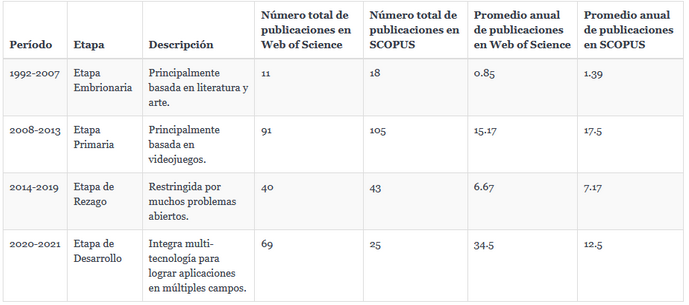
\includegraphics[width=0.7\textwidth]{tablaPublicaciones.PNG}
		\caption{Descripción de la imagen}
		\label{fig:tabla_publicaciones}
	\end{figure} \\
	Actualmente estamos en la etapa de desarrollo donde se están integrando y desarrollando diferentes tecnologías para la creación del Metaverso.  Estas tecnologías se pueden dividir en cinco aspectos: infraestructura de red, tecnología de gestión, tecnología común básica, conexión de objeto de realidad virtual y convergencia de realidad virtual. Una breve descripción de las tecnologías involucradas es la siguiente:
	\begin{enumerate}
		\item \textbf{Infraestructura de comunicación y computación:} Se refiere a las bases tecnológicas que hacen posible el Metaverso, principalmente las redes 5G y 6G. Estas redes ofrecen alta velocidad, baja latencia y conectividad ubicua. La comunicación cuántica garantiza la seguridad en este entorno. Además, el Internet de las Cosas (IoT) es esencial para conectar el Metaverso con el mundo real. La computación en la nube y en el borde son fundamentales para proporcionar la potencia informática necesaria.
		
		\item \textbf{Tecnología de Gestión:} Se centra en cómo se gestionan y mantienen los recursos dentro del Metaverso. Esto incluye la gestión de la energía utilizada por las instalaciones del Metaverso, la asignación y descubrimiento de recursos y la gestión de las interacciones de los usuarios en sesiones. La seguridad y la prevención de ataques también son consideraciones clave en este ámbito.
		
		\item \textbf{Tecnologías fundamentales:} Son las tecnologías esenciales que respaldan las operaciones y el desarrollo del Metaverso. Estas incluyen la realidad virtual y aumentada, la inteligencia artificial, la visión por computadora y la tecnología blockchain. Estas tecnologías permiten la creación de mundos virtuales y la interacción dentro de ellos. Entre ellas IA con frameworks como TensorFlow, permitiendo interacciones avanzadas, lenguajes como Solidity respalda contratos inteligentes y transacciones seguras.
		
		\item \textbf{Conexión de Objetos de Realidad Virtual:} Trata sobre cómo los objetos virtuales en el Metaverso interactúan entre sí y con los usuarios. Esto abarca desde la creación de objetos hasta su interacción y eventual destrucción, todo lo cual contribuye a una experiencia inmersiva para los usuarios.
		
		\item \textbf{Convergencia de Realidad Virtual:} Se refiere a la interacción entre el mundo virtual del Metaverso y el mundo real. Esto incluye cómo la información se mueve entre estos dos mundos, cómo los usuarios pueden transitar entre ellos y cómo las acciones en uno pueden influir en el otro. Por ejemplo, cómo las tecnologías AR (Augmented Reality), VR (Virtual Reality), MR (Mixed Reality).
		
	\end{enumerate}
	\subsection{Importancia y futuro del metaverso}
	La creación de diversas tecnologías que impulsan y adoptan el metaverso como la realidad virtual (VR), realidad aumentada (AR) entre otras. Nos permite visualizar nuevos mercados y formas de entretenimiento que antes no existían o eran de nicho, el comercio de bienes virtuales, la posesión y alquiler de tierras digitales, son nuevos mercados no explorados, los juegos en VR, vivir eventos históricos, etc. El metaverso se está desarrollando relativamente rápido, sin embargo, todavía quedan problemas abiertos por resolver. Ejemplos de estos problemas son los siguientes: problemas de cómputo (el procesamiento de datos), éticos (controlar y restringir el comportamiento de los usuarios, establecer normas éticas), el síndrome cibernético (trastorno físico, social y mental causado por el uso excesivo de internet), por último los problemas de estándares y compatibilidad (compatibilidad entre metaversos creados por diferentes empresas y compatibilidad entre metaversos-mundo real).
	
	\section{Inteligencia Artificial y Blockchain en el Metaverso}
	Tenga en cuenta que, en este trabajo no desarrollaremos conceptos como VR, AR y relacionados con la inmersión. Debido a que este trabajo está enfocado al lenguaje de programación Solidity (se puede decir que es el backend del metaverso) relacionado a la smart contract, blockchain e inteligencia artificial.
	\subsection{Inteligencia artificial}
	\subsection{Blockchain y Smart Contracts}
	\section{Solidity}
	\nocite{*}
	\printbibliography[heading=bibintoc]
\end{document}
